\scanpage{85}
\mspage{- 538 -}

\begin{center}
TABLE OF CONTENTS
\end{center}

\noindent FOREWORD \dotfill

\noindent INTRODUCTION\dotfill

\noindent CHAPTER \unsure{O|0} .- Preliminaries\dotfill

\noindent\quad \S\ 1. Representable functors\dotfill

\noindent\qquad 1.1. Representable functors\dotfill

\noindent\qquad 1.2. Fiber products in a category\dotfill

\noindent\qquad 1.3. Base change\dotfill

\noindent\qquad 1.4. Kernels ; diagonal morphism\dotfill

\noindent\qquad 1.5. Adjoint functors\dotfill

\noindent\qquad 1.6. Algebraic structures in categories\dotfill

\noindent\qquad 1.7. Representable functorial morphisms\dotfill

\noindent\quad \S\ 2. Complements on topology\dotfill

\noindent\qquad 2.1. Irreducible spaces\dotfill

\noindent\qquad 2.2. Locally noetherian spaces\dotfill

\noindent\qquad 2.3. Quasi-constructible sets and constructible sets\dotfill

\begingroup
\reversemarginpar
\margin{\figure{\handwritten{\unsure{%
\begin{tikzpicture}[x=1mm,y=1mm]
\draw[line width=0.5pt]
 (0,6.80) .. controls (0.50,7.00) and (1.15,7.25) .. (1.62,7.15)
 .. controls (2.05,7.06) and (2.23,6.60) .. (2.13,6.12)
 .. controls (2.05,5.10) and (1.77,4.02) .. (1.46,2.77)
 .. controls (1.32,2.40) and (1.37,2.15) .. (1.69,2.10)
 .. controls (2.02,2.02) and (2.30,2.36) .. (2.55,2.18);
\draw[line width=0.5pt] (3.34,0.15) .. controls (3.64,0.28) and (3.91,0.22) .. (4.10,0.16);
\end{tikzpicture}%
}}}}
\endgroup
\figure{%
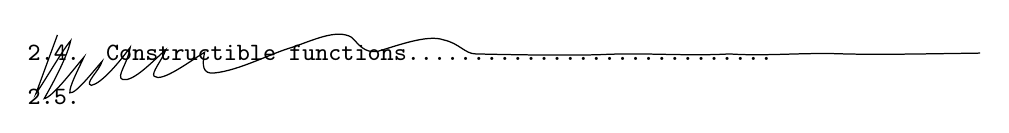
\begin{tikzpicture}[x=0.105mm,y=-0.105mm]
\node[anchor=base west,inner sep=0pt,outer sep=0pt,font=\ttfamily\small] at (13,41)
 {\deleted{2.4. Constructible functions}\deleted{\mbox{............................}}};
\node[anchor=base west,inner sep=0pt,outer sep=0pt,font=\ttfamily\small] at (13,94)
 {\deleted{2.5.}};
% The deletion macros record state; this path records the observed freehand course.
\handwritten{\draw[line width=0.45pt]
 (49,10) -- (23,81)
 .. controls (31,70) and (56,27) .. (65,17)
 .. controls (60,40) and (38,78) .. (33,87)
 .. controls (43,86) and (72,47) .. (81,37)
 .. controls (74,52) and (63,73) .. (64,80)
 .. controls (71,82) and (93,53) .. (103,42)
 .. controls (100,53) and (81,69) .. (90,71)
 .. controls (102,69) and (124,43) .. (137,25)
 .. controls (135,43) and (119,61) .. (128,64)
 .. controls (141,67) and (164,42) .. (180,28)
 .. controls (176,40) and (162,56) .. (166,60)
 .. controls (175,68) and (209,42) .. (227,31)
 .. controls (224,46) and (224,58) .. (239,56)
 .. controls (269,53) and (308,32) .. (333,25)
 .. controls (357,17) and (387,2) .. (405,13)
 .. controls (414,22) and (420,32) .. (436,30)
 .. controls (460,23) and (497,9) .. (516,16)
 .. controls (535,20) and (542,33) .. (555,33)
 .. controls (601,34) and (652,35) .. (703,34)
 .. controls (758,31) and (808,36) .. (862,33)
 .. controls (906,36) and (951,31) .. (1001,33)
 .. controls (1046,34) and (1093,33) .. (1165,32);}
\end{tikzpicture}%
}

\noindent\qquad 2.4. Constructible sets in noetherian spaces

\noindent\qquad 2.5? Constructible functions\dotfill

\noindent\qquad 2.6. Very dense subsets of a topological space\dotfill

\noindent\qquad 2.7. Quasi-homeomorphisms\dotfill

\noindent\qquad 2.8. Jacobson spaces\dotfill

\noindent\qquad 2.9. Sober space associated with a topological space\dotfill

\noindent\qquad 2.10.Maps open at a point \dotfill

\noindent\quad \S\ 3. Complements on sheaves\dotfill

\noindent\qquad 3.1. Sheaves with values in a category\dotfill

\noindent\qquad 3.2. Presheaves on a basis of open sets\dotfill

\noindent\qquad 3.3. Gluing of sheaves\dotfill

\noindent\qquad 3.4. Direct images of presheaves\dotfill

\noindent\qquad 3.5. Inve\deleted{\unsure{r}}r\deleted{p}se image\unsure{s|\deleted{s}s|ss} of presheaves\dotfill

\noindent\qquad 3.6. Simple sheaves and locally simple sheaves\dotfill

\noindent\qquad 3.7. Inverse images of sheaves of groups or rings\dotfill

% archive sheet number: 84
\clearpage
